\documentclass{article}

% Language setting
% Replace `english' with e.g. `spanish' to change the document language
\usepackage[english]{babel}

% Set page size and margins
% Replace `letterpaper' with`a4paper' for UK/EU standard size
\usepackage[letterpaper,top=2cm,bottom=2cm,left=3cm,right=3cm,marginparwidth=1.75cm]{geometry}

% Useful packages
\usepackage{amsmath}
\usepackage{graphicx}
\usepackage[colorlinks=true, allcolors=blue]{hyperref}
\usepackage{tabularx}
\usepackage{fvextra}
\usepackage{ulem}


\usepackage{array,multirow,makecell}

\usepackage{graphicx}
\usepackage{subcaption}
\usepackage{xparse}

\usepackage{graphicx}
\usepackage{subcaption}
\usepackage{xparse}

\usepackage{placeins}

\NewDocumentCommand{\DoubleFigure}{m m m m m m m}{
\begin{figure}[ht]
    \centering

    \begin{subfigure}{0.48\textwidth}
        \centering
        \includegraphics[width=\linewidth]{#1}
        \caption{#2}
        \label{#3}
    \end{subfigure}
    \hfill
    \begin{subfigure}{0.48\textwidth}
        \centering
        \includegraphics[width=\linewidth]{#4}
        \caption{#5}
        \label{#6}
    \end{subfigure}

    \caption{#7}
\end{figure}
}

\setcellgapes{1pt}
\makegapedcells
\newcolumntype{R}[1]{>{\raggedleft\arraybackslash }b{#1}}
\newcolumntype{L}[1]{>{\raggedright\arraybackslash }b{#1}}
\newcolumntype{C}[1]{>{\centering\arraybackslash }b{#1}}

\title{Rapport d'avancement}
\author{Vital FOCHEUX}
\date{du 18 juin au 26 juin}

\begin{document}

\maketitle

\section{Notes de la dernière réunion}

\begin{itemize}
    \item Essayer les filtres passe-bas et passe-haut avec un signal plus réaliste
    \item Refaire les résultats du filtre passe-bas avec une fréquence de coupure plus proche du signal voulu
    \item Refaire les plots sur les anti-windups en ayant la courbe sans anti-windup en pointillés pour mieux voir la différence
    \item Continuer la rédaction du rapport de stage
\end{itemize}

\section{Depuis la dernière fois}

\subsection{Filtre passe-bas}

J'ai refait les plots du filtre passe-bas avec une fréquence de coupure plus proche du signal voulu.
Les fréquences sont de 10 Hz pour celle voulu et 200 Hz pour le bruit et la fréquence de coupure du 
filtre est de 15 Hz.

\DoubleFigure
    {low_pass_order1.png}
    {Filtre passe-bas ordre 1 avec une fréquence de coupure de 15 Hz}
    {fig:lowpass_ordre1_15}
    {low_pass_order1 (2).png}
    {Filtre passe-bas ordre 1 avec une fréquence de coupure de 50 Hz}
    {fig:lowpass_ordre1_50}
    {Comparaison des résultats du filtre passe-bas d'ordre 1 avec deux fréquences de coupure différentes}

\DoubleFigure
    {low_pass_fft_order1.png}
    {Spectre fréquentiel du signal avant et après filtre passe-bas d'ordre 1 avec une fréquence de coupure de 15 Hz}
    {fig:low_pass_fft_order1_15}
    {low_pass_fft_order1 (2).png}
    {Spectre fréquentiel du signal avant et après filtre passe-bas d'ordre 1 avec une fréquence de coupure de 50 Hz}
    {fig:low_pass_fft_order1_50}
    {Comparaison des spectres fréquentiels du signal avant et après filtre passe-bas d'ordre 1 avec deux fréquences de coupure différentes}

\DoubleFigure
    {low_pass_psd_order1.png}
    {Densité spectrale de puissance avant et après filtre passe-bas d'ordre 1 avec une fréquence de coupure de 15 Hz}
    {fig:low_pass_psd_order1_15}
    {low_pass_psd_order1 (2).png}
    {Densité spectrale de puissance avant et après filtre passe-bas d'ordre 1 avec une fréquence de coupure de 50 Hz}
    {fig:low_pass_psd_order1_50}
    {Comparaison des densités spectrales de puissance du signal avant et après filtre passe-bas d'ordre 1 avec deux fréquences de coupure différentes}

\DoubleFigure
    {low_pass_order2.png}
    {Filtre passe-bas d'ordre 2 avec une fréquence de coupure de 15 Hz}
    {fig:low_pass_order2_15}
    {low_pass_order2 (2).png}
    {Filtre passe-bas d'ordre 2 avec une fréquence de coupure de 50 Hz}
    {fig:low_pass_order2_50}
    {Comparaison des résultats du filtre passe-bas d'ordre 2 avec deux fréquences de coupure différentes}

\DoubleFigure
    {low_pass_fft_order2.png}
    {Spectre fréquentiel du signal avant et après filtre passe-bas d'ordre 2 avec une fréquence de coupure de 15 Hz}
    {fig:low_pass_fft_order2_15}
    {low_pass_fft_order2 (2).png}
    {Spectre fréquentiel du signal avant et après filtre passe-bas d'ordre 2 avec une fréquence de coupure de 50 Hz}
    {fig:low_pass_fft_order2_50}
    {Comparaison des spectres fréquentiels du signal avant et après filtre passe-bas d'ordre 2 avec deux fréquences de coupure différentes}

\DoubleFigure
    {low_pass_psd_order2.png}
    {Densité spectrale de puissance avant et après filtre passe-bas d'ordre 2 avec une fréquence de coupure de 15 Hz}
    {fig:low_pass_psd_order2_15}
    {low_pass_psd_order2 (2).png}
    {Densité spectrale de puissance avant et après filtre passe-bas d'ordre 2 avec une fréquence de coupure de 50 Hz}
    {fig:low_pass_psd_order2_50}
    {Comparaison des densités spectrales de puissance du signal avant et après filtre passe-bas d'ordre 2 avec deux fréquences de coupure différentes}

\FloatBarrier

\newpage

\subsection{Instuments}

J'ai réalisé un test avec un signal plus réaliste pour les filtres passe-bas et passe-haut. Le signal est un mélange de trois instruments différents : 
une basse, une guitare électrique et une flûte, qui dure au total 4 secondes. 

L'objectif est de filtrer le signal de chaque instrument avec un filtre passe-bas et un filtre passe-haut. 
Pour filtrer le signal de la basse, les fréquences de coupures sont de 250 Hz pour le filtre passe-bas et 30 Hz 
pour le filtre passe-haut.
Pour filtrer le signal de la guitare électrique, les fréquences de coupures sont de 900 Hz pour le filtre passe-bas et 
280 Hz pour le filtre passe-haut.
Pour filtrer le signal de la flûte, les fréquences de coupures sont de 1400 Hz pour le filtre passe-bas et 1000 Hz 
pour le filtre passe-haut.

Les fréquences de coupures ont été choisies en fonction des fréquences de chaque intrument, qu'on trouve 
\href{https://www.studioenregistrement.fr/post/frequences-des-instruments-de-musique}{ici}, il a fallu adapter 
avec l'exemple car on peut distinguer les fréquences de chaque instrument dans le spectre fréquentiel du signal.


\begin{figure}[h]
    \centering
    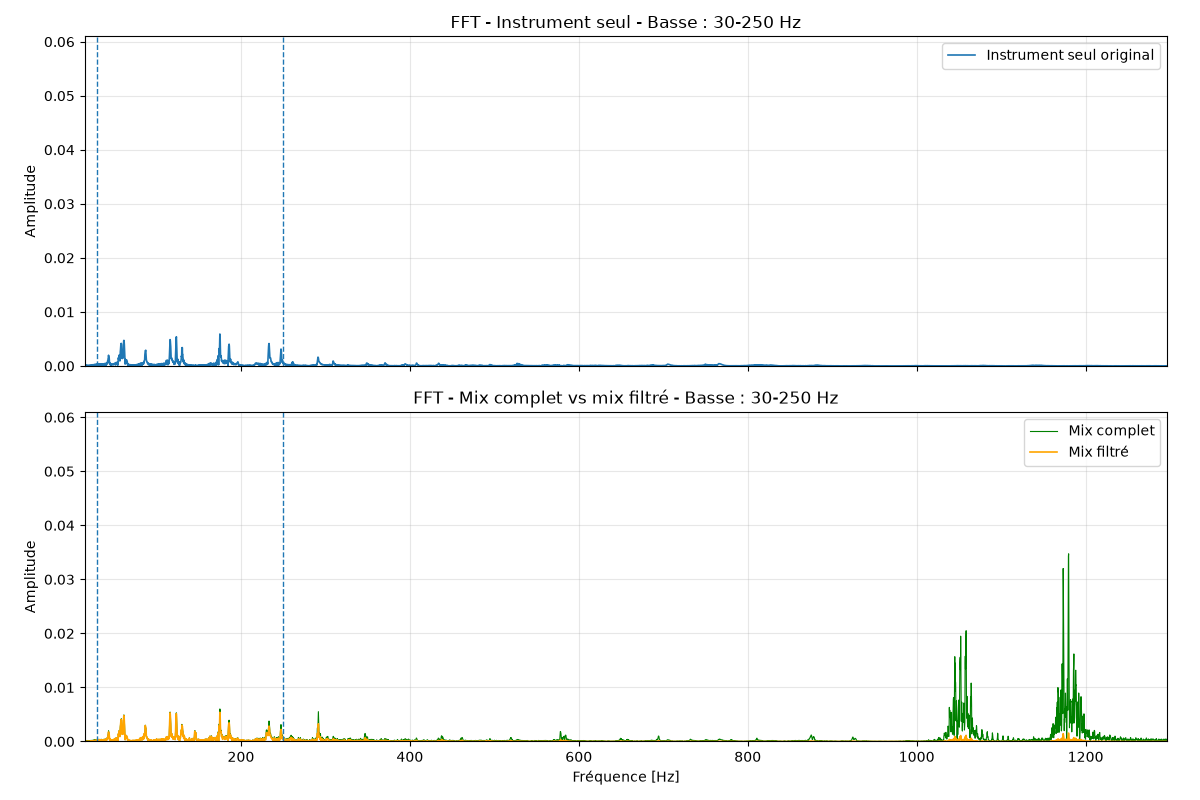
\includegraphics[width=\textwidth]{bass_fft.png}
    \caption{Spectre fréquentiel du signal de la basse}
    \label{fig:bass_fft}
\end{figure}

\begin{figure}[h]
    \centering
    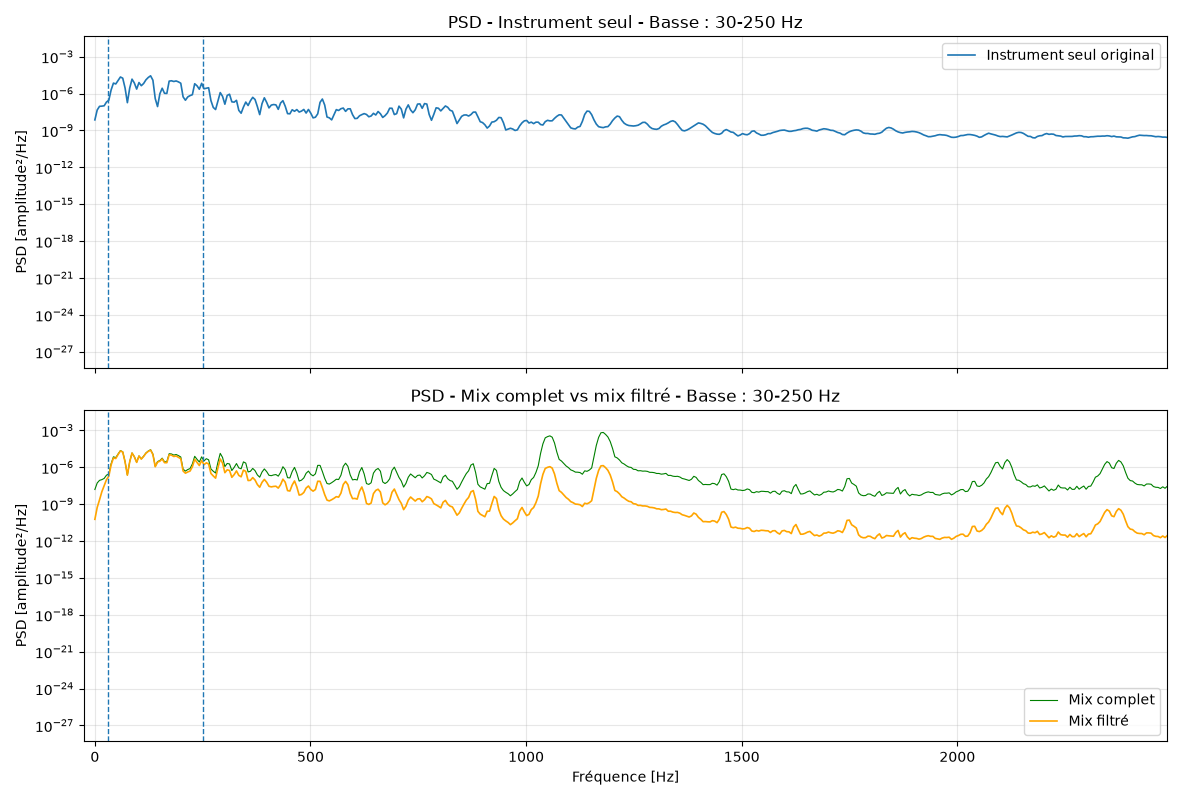
\includegraphics[width=\textwidth]{bass_psd.png}
    \caption{Densité spectrale de puissance du signal de la basse}
    \label{fig:bass_psd}
\end{figure}

\begin{figure}[h]
    \centering
    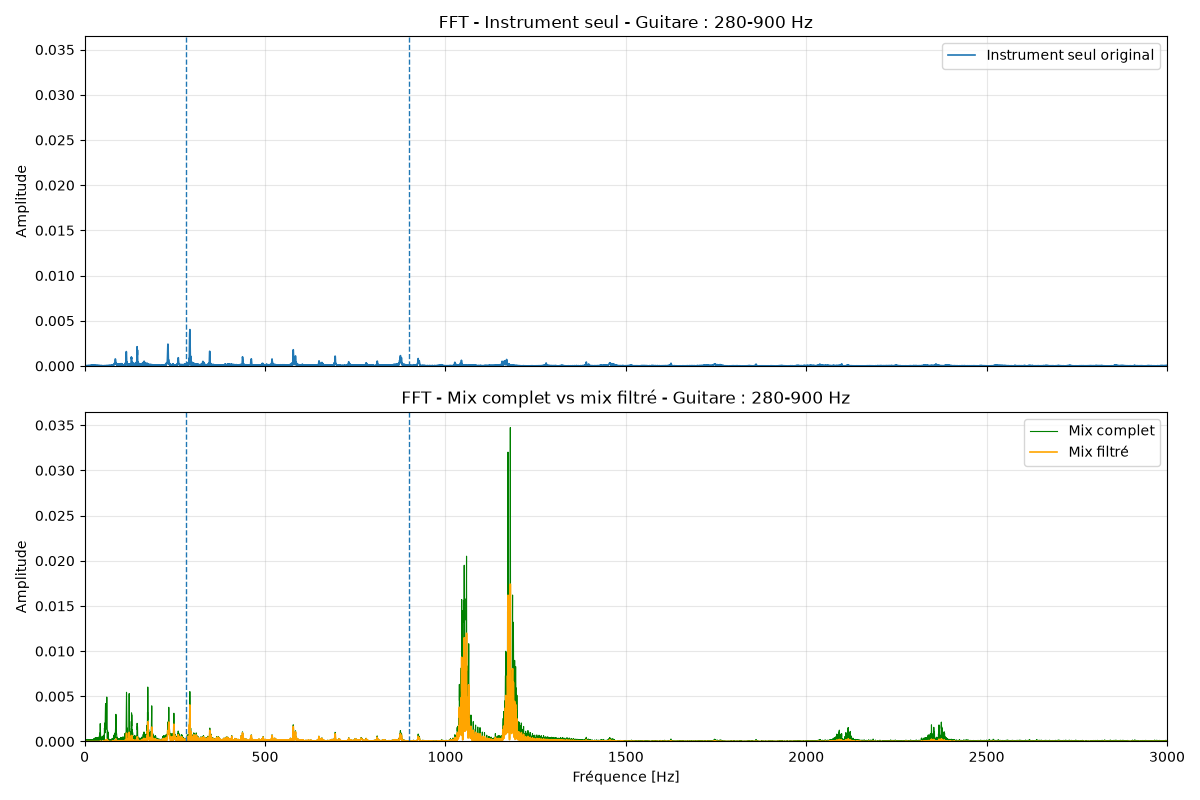
\includegraphics[width=\textwidth]{guitar_fft.png}
    \caption{Spectre fréquentiel du signal de la guitare électrique}
    \label{fig:guitar_fft}
\end{figure}

\begin{figure}[h]
    \centering
    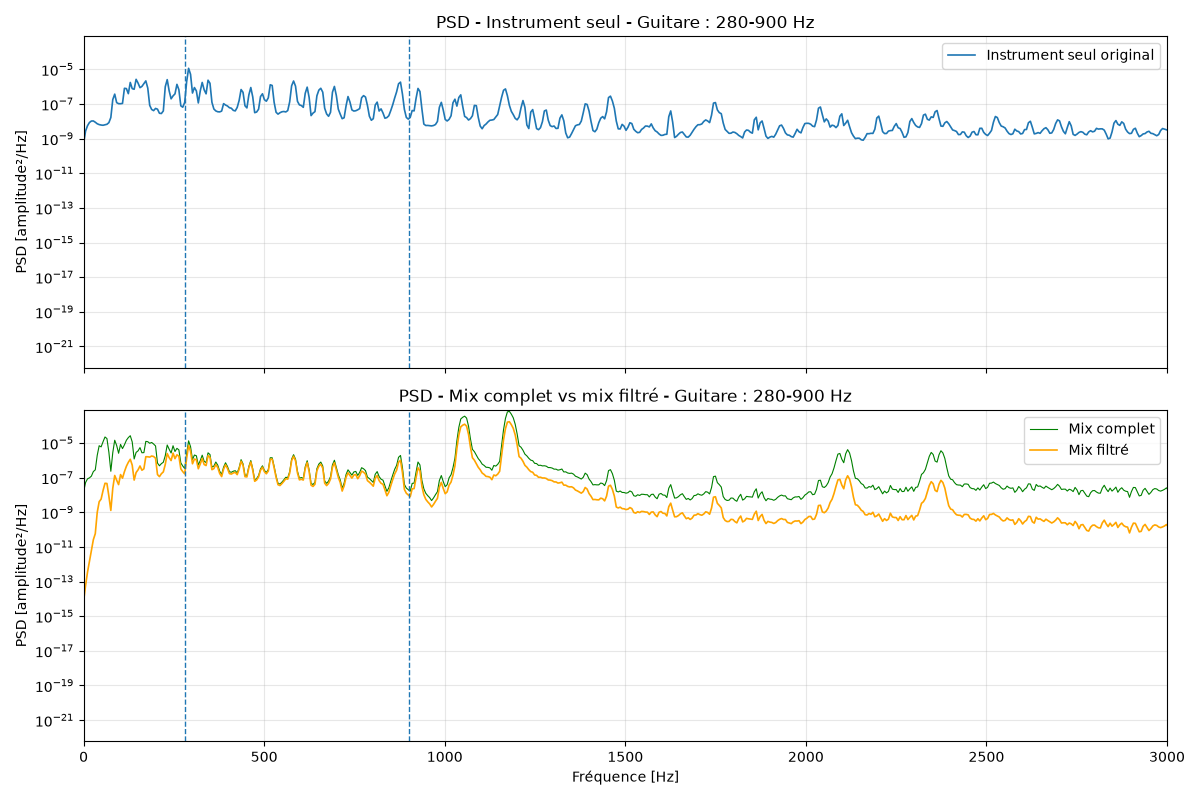
\includegraphics[width=\textwidth]{guitar_psd.png}
    \caption{Densité spectrale de puissance du signal de la guitare électrique}
    \label{fig:guitar_psd}
\end{figure}

\begin{figure}
    \centering
    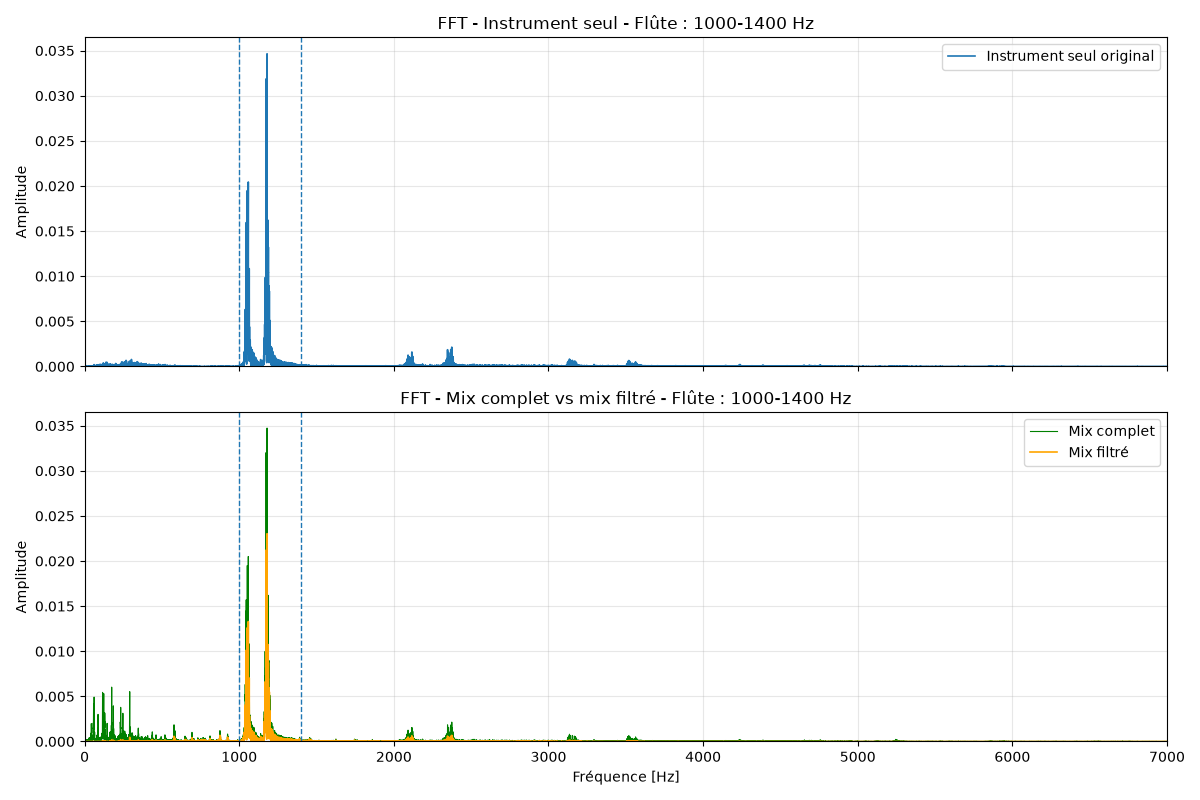
\includegraphics[width=\textwidth]{flute_fft.png}
    \caption{Spectre fréquentiel du signal de la flûte}
    \label{fig:flute_fft}
\end{figure}

\begin{figure}
    \centering
    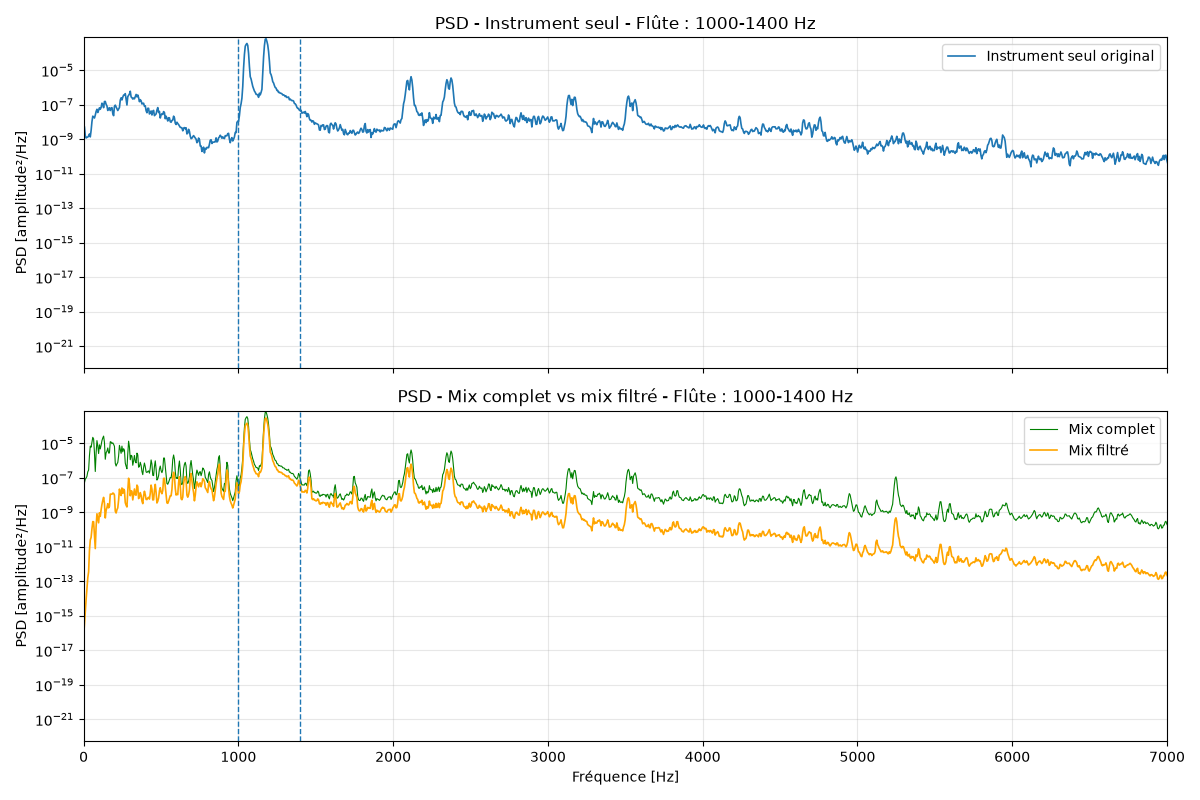
\includegraphics[width=\textwidth]{flute_psd.png}
    \caption{Densité spectrale de puissance du signal de la flûte}
    \label{fig:flute_psd}
\end{figure}

\FloatBarrier

\newpage

\subsection{Rapport}

J'ai continué la rédaction du rapport de stage, un brouillon a été envoyé par mail mercredi 1 juillet où 
les parties 1, 3 et 6 sont à compléter. Pour les autres parties, le manque principal est celui de schémas et 
d'autres illustrations pour mieux comprendre les explications. 

\end{document}